\documentclass[11pt,a4paper]{article}

% === Encodage ===
\usepackage[utf8]{inputenc}
\usepackage[T1]{fontenc}

% === Mise en page ===
\usepackage[margin=2.2cm]{geometry}
\usepackage{fancyhdr}
\usepackage{lastpage}

% === Math et unités ===
\usepackage{amsmath,amssymb}
\usepackage{siunitx}
\sisetup{
  locale = FR,
  group-separator = {\,},
  output-decimal-marker = {,},
  per-mode = symbol,
}

% === Tableaux ===
\usepackage{booktabs}
\usepackage{multirow}
\usepackage{array}
\usepackage{colortbl}

% === Figures ===
\usepackage{graphicx}
\usepackage[dvipsnames,table]{xcolor}
\usepackage{tikz}
\usetikzlibrary{arrows.meta,patterns,decorations.pathmorphing,calc,positioning}
\usepackage{caption}
\usepackage{float}

% === Divers ===
\usepackage{enumitem}
\usepackage{pifont}
\usepackage{hyperref}
\hypersetup{
  colorlinks=true,
  linkcolor=NavyBlue,
  citecolor=ForestGreen,
  urlcolor=RoyalBlue,
}

% === En-tête / pied de page ===
\pagestyle{fancy}
\fancyhf{}
\lhead{\small\textsc{Concept de lentille Compton en graphite}}
\rhead{\small Simulation Geant4 --- MiniX}
\cfoot{\small Page \thepage/\pageref{LastPage}}
\renewcommand{\headrulewidth}{0.4pt}
\renewcommand{\footrulewidth}{0.2pt}

% === Couleurs ===
\definecolor{graphite}{RGB}{44,62,80}
\definecolor{brass}{RGB}{212,160,23}
\definecolor{comptonblue}{RGB}{41,128,185}
\definecolor{photored}{RGB}{231,76,60}

% ======================================================================
\title{%
  \vspace{-1.5cm}
  {\Large\textsc{Proposition de configuration}}\\[0.3cm]
  {\LARGE\bfseries Collimateur conique concentrateur Compton\\en graphite}\\[0.3cm]
  {\large\itshape Remplacement du syst\`eme Al\,+\,Laiton par un
  c\^one en carbone pour la focalisation de rayons X}
}
\author{%
  Application : tube Amptek MiniX (\SIrange{1}{50}{\kilo\electronvolt}, c\^one 60$^\circ$)
}
\date{\today}

\begin{document}
\maketitle
\thispagestyle{fancy}

% ======================================================================
\section{Motivation et probl\'ematique}
% ======================================================================

Le tube \`a rayons X Amptek MiniX \'emet un faisceau divergent dans un c\^one de demi-angle
60$^\circ$. Le syst\`eme de collimation actuel (tube aluminium + tube laiton, bore
cylindrique $\varnothing$\,\SI{3}{\milli\metre}) ne transmet que \SI{0,78}{\percent} des
photons primaires (run de r\'ef\'erence, \num{5000000}~\'ev\'enements). Les
\SI{99,2}{\percent} restants sont absorb\'es par effet photo\'electrique, principalement
dans le laiton (\SI{60,5}{\percent}) et l'aluminium (\SI{33}{\percent}).

\medskip
\noindent\textbf{Objectif~:} transformer le syst\`eme de collimation en
\textbf{concentrateur}, capable de rediriger les photons \`a grand angle vers l'axe du
faisceau, m\^eme au prix d'une l\'eg\`ere perte d'\'energie. Le porte-collimateur en
inox\,304 est impos\'e et ne peut \^etre modifi\'e.

\medskip
\noindent\textbf{Id\'ee~:} exploiter la \textbf{diffusion Compton} dans un mat\'eriau de
bas num\'ero atomique $Z$ comme m\'ecanisme de redirection, en rempla\c{c}ant les tubes
m\'etalliques par un c\^one unique en \textbf{graphite} (carbone, $Z = 6$).

% ======================================================================
\section{Fondements physiques}
\label{sec:physics}
% ======================================================================

\subsection{Cin\'ematique de la diffusion Compton}

La diffusion Compton est la collision d'un photon avec un \'electron quasi-libre. L'\'energie
du photon diffus\'e est donn\'ee par~:
\begin{equation}
  \boxed{
  E' \;=\; \frac{E}{1 + \dfrac{E}{m_e c^2}\,(1 - \cos\theta)}
  }
  \label{eq:compton}
\end{equation}
o\`u $E$ est l'\'energie incidente, $\theta$ l'angle de diffusion et
$m_e c^2 = \SI{511}{\kilo\electronvolt}$. \`A basse \'energie ($E \ll m_e c^2$), on se
trouve dans le \textbf{r\'egime Thomson}~: la perte d'\'energie est n\'egligeable.

Le tableau~\ref{tab:eloss} quantifie la perte d'\'energie pour le spectre du MiniX~:

\begin{table}[H]
\centering
\caption{Perte d'\'energie Compton $\Delta E / E$ (\%) pour diff\'erents angles et \'energies.}
\label{tab:eloss}
\begin{tabular}{@{}r S[table-format=1.1] S[table-format=1.1]
                    S[table-format=1.1] S[table-format=2.1]@{}}
\toprule
{$E$ (keV)} & {$\theta = 30^\circ$} & {$\theta = 60^\circ$}
            & {$\theta = 90^\circ$} & {$\theta = 180^\circ$} \\
\midrule
5  & 0.1 & 0.5 & 1.0 & 1.9 \\
10 & 0.3 & 1.0 & 1.9 & 3.8 \\
20 & 0.5 & 1.9 & 3.8 & 7.3 \\
50 & 1.3 & 4.7 & 8.9 & 16.4 \\
\bottomrule
\end{tabular}
\end{table}

\noindent\textbf{Point cl\'e~:} \`a \SI{10}{\kilo\electronvolt}, m\^eme une
r\'etrodiffusion compl\`ete ($\theta = 180^\circ$) ne co\^ute que \SI{3,8}{\percent}
d'\'energie. Le Compton fonctionne ici comme une \textbf{r\'eflexion quasi-\'elastique}.

\begin{figure}[H]
\centering
\includegraphics[width=\textwidth]{fig_compton_kinematics.pdf}
\caption{\textbf{(a)}~Perte d'\'energie relative $\Delta E / E$ en fonction de l'angle de
  diffusion pour plusieurs \'energies incidentes. \`A \SI{10}{\kilo\electronvolt},
  $\Delta E < \SI{2}{\percent}$ pour $\theta < 90^\circ$.
  \textbf{(b)}~Section efficace diff\'erentielle de Klein-Nishina (normalis\'ee). \`A basse
  \'energie la distribution est quasi-isotrope (limite de Thomson), ce qui signifie
  qu'environ 50\% des diffusions se font dans l'h\'emisph\`ere avant.}
\label{fig:kinematics}
\end{figure}

\subsection{Distribution angulaire~: la formule de Klein-Nishina}

La section efficace diff\'erentielle est donn\'ee par~:
\begin{equation}
  \frac{\mathrm{d}\sigma}{\mathrm{d}\Omega} = \frac{r_e^2}{2}\,P(\theta)^2
  \left[ P(\theta) + \frac{1}{P(\theta)} - \sin^2\theta \right]
  \quad\text{avec}\quad
  P(\theta) = \frac{1}{1 + \alpha\,(1 - \cos\theta)}
  \label{eq:KN}
\end{equation}
o\`u $\alpha = E / (m_e c^2)$ et $r_e = \SI{2,818e-13}{\centi\metre}$. Comme le montre la
figure~\ref{fig:kinematics}b, \`a nos \'energies ($\alpha < 0{,}1$) la distribution est
quasi-isotrope. Cela signifie que $\sim$\textbf{50\% des interactions Compton} produiront un
photon diffus\'e dans l'h\'emisph\`ere avant, exploitable pour la concentration.

\medskip
\noindent\fbox{\parbox{0.97\linewidth}{
\textbf{R\'esum\'e physique~:} entre \SIrange{5}{50}{\kilo\electronvolt}, la diffusion
Compton est \textbf{(i)}~quasi-\'elastique ($\Delta E/E < 4\%$) et
\textbf{(ii)}~quasi-isotrope ($\sim$50\% forward). C'est un m\'ecanisme id\'eal pour
\textbf{rediriger} des photons sans les d\'etruire.
}}

% ======================================================================
\section{Choix du mat\'eriau}
\label{sec:material}
% ======================================================================

\subsection{Crit\`eres de s\'election}

Pour que la diffusion Compton domine l'absorption photo\'electrique, il faut~:
\begin{enumerate}[nosep,leftmargin=2em]
  \item \textbf{$Z$ bas} --- $\sigma_{\text{photo}} \propto Z^{4\text{--}5}$ tandis que
    $\sigma_{\text{Compton}} \propto Z$. Passer de $Z = 29$ (laiton) \`a $Z = 6$ (carbone)
    r\'eduit le rapport photo/Compton d'un facteur
    $\sim (29/6)^4 \approx 550$.
  \item \textbf{Densit\'e suffisante} --- pour obtenir une probabilit\'e d'interaction
    significative dans $\sim$\SI{2}{\milli\metre} de paroi.
  \item \textbf{Tenue m\'ecanique et thermique} --- usinabilit\'e, r\'esistance
    \`a l'environnement du tube X.
\end{enumerate}

\subsection{Comparaison des mat\'eriaux candidats}

\begin{figure}[H]
\centering
\includegraphics[width=\textwidth]{fig_materiaux_comparaison.pdf}
\caption{\textbf{(a)}~Fraction de l'att\'enuation lin\'eique due au Compton.
  Le graphite et le b\'eryllium atteignent les fractions les plus \'elev\'ees au-dessus de
  \SI{10}{\kilo\electronvolt}. Le laiton reste domin\'e par le photo\'electrique sur tout le
  spectre.
  \textbf{(b)}~Probabilit\'e de diffusion Compton dans \SI{2,1}{\milli\metre} de paroi. Le
  graphite offre la probabilit\'e la plus \'elev\'ee en valeur absolue gr\^ace \`a sa
  densit\'e ($\rho = \SI{2,26}{\gram\per\centi\metre\cubed}$).}
\label{fig:materials}
\end{figure}

\begin{table}[H]
\centering
\caption{Propri\'et\'es des mat\'eriaux candidats pour le c\^one Compton
  (\SI{2,1}{\milli\metre} de paroi, $E = \SI{10}{\kilo\electronvolt}$).}
\label{tab:materials}
\small
\begin{tabular}{@{}l c c c c l@{}}
\toprule
\textbf{Mat\'eriau} & $Z_{\text{eff}}$ & $\rho$ (g/cm$^3$)
  & $P_{\text{Compt}}$ & $P_{\text{photo}}$ & \textbf{Remarques} \\
\midrule
\rowcolor{graphite!10}
\textbf{Graphite (C)} & \textbf{6} & \textbf{2,26} & \textbf{6,0\%} & 32\%
  & \textbf{Meilleur compromis} \\
B\'eryllium (Be) & 4 & 1,85 & 4,2\% & 0,4\%
  & Toxique, co\^uteux \\
PMMA & 6,5 & 1,19 & 3,4\% & 14\%
  & Fond \`a 160\,$^\circ$C \\
Poly\'ethyl\`ene & 5,5 & 0,94 & 2,9\% & 7\%
  & Trop l\'eger, mou \\
B$_4$C & 5,2 & 2,52 & 4,5\% & 18\%
  & Tr\`es dur \`a usiner \\
\midrule
Laiton (r\'ef.) & 29 & 8,73 & $\ll 0{,}1$\% & $> 99{,}9$\%
  & Tout est absorb\'e \\
\bottomrule
\end{tabular}
\end{table}

\paragraph{Conclusion~:} le \textbf{graphite} (\texttt{G4\_GRAPHITE},
$\rho = \SI{2,26}{\gram\per\centi\metre\cubed}$, $Z = 6$) est le meilleur candidat. Il
combine~:
\begin{itemize}[nosep,leftmargin=2em]
\item le meilleur taux de Compton absolu (gr\^ace \`a sa densit\'e \'elev\'ee parmi les bas-$Z$),
\item une suppression forte du photo\'electrique ($Z^4$ bas),
\item une excellente tenue thermique ($> \SI{3000}{\celsius}$ sous atmosph\`ere inerte),
\item une bonne usinabilit\'e.
\end{itemize}

\subsection{Devenir d'un photon dans le graphite}

\begin{figure}[H]
\centering
\includegraphics[width=0.8\textwidth]{fig_devenir_photons_graphite.pdf}
\caption{R\'epartition du devenir d'un photon traversant environ \SI{3}{\milli\metre} de
  graphite (chemin effectif pour incidence rasante dans le c\^one). \`A
  \SI{10}{\kilo\electronvolt}, environ 8\% subissent un Compton, 60\% sont
  photo-absorb\'es et 32\% traversent sans interaction. Au-del\`a de
  \SI{20}{\kilo\electronvolt}, le Compton devient le processus d'interaction dominant.}
\label{fig:fate}
\end{figure}

% ======================================================================
\section{G\'eom\'etrie propos\'ee~: le c\^one concentrateur}
\label{sec:geometry}
% ======================================================================

\subsection{Principe de fonctionnement}

L'id\'ee est de remplacer le bore cylindrique (Al + Laiton) par un \textbf{bore conique}
en graphite, \'elas\'e c\^ot\'e source et r\'etr\'eci c\^ot\'e d\'etecteur
(figure~\ref{fig:schema}). Le c\^one agit en trois zones~:

\begin{enumerate}[nosep,leftmargin=2em]
  \item \textbf{Zone de transmission directe} ($\theta < 3{,}2^\circ$)~: les photons
    traversent le bore sans interaction $\longrightarrow$ faisceau primaire inchang\'e.

  \item \textbf{Zone de capture Compton} ($3{,}2^\circ < \theta < 30^\circ$)~: les photons
    frappent la paroi interne du c\^one en graphite sous \textbf{incidence rasante},
    traversant un chemin effectif de \SIrange{3}{15}{\milli\metre}. Une fraction
    significative subit une diffusion Compton et est redirig\'ee vers l'avant avec
    $> \SI{98}{\percent}$ de son \'energie.

  \item \textbf{Zone d'absorption} ($\theta > 30^\circ$)~: les photons traversent le
    graphite (trop mince \`a l'entr\'ee) et sont absorb\'es par le porte-collimateur inox.
\end{enumerate}

\begin{figure}[H]
\centering
\resizebox{\textwidth}{!}{%
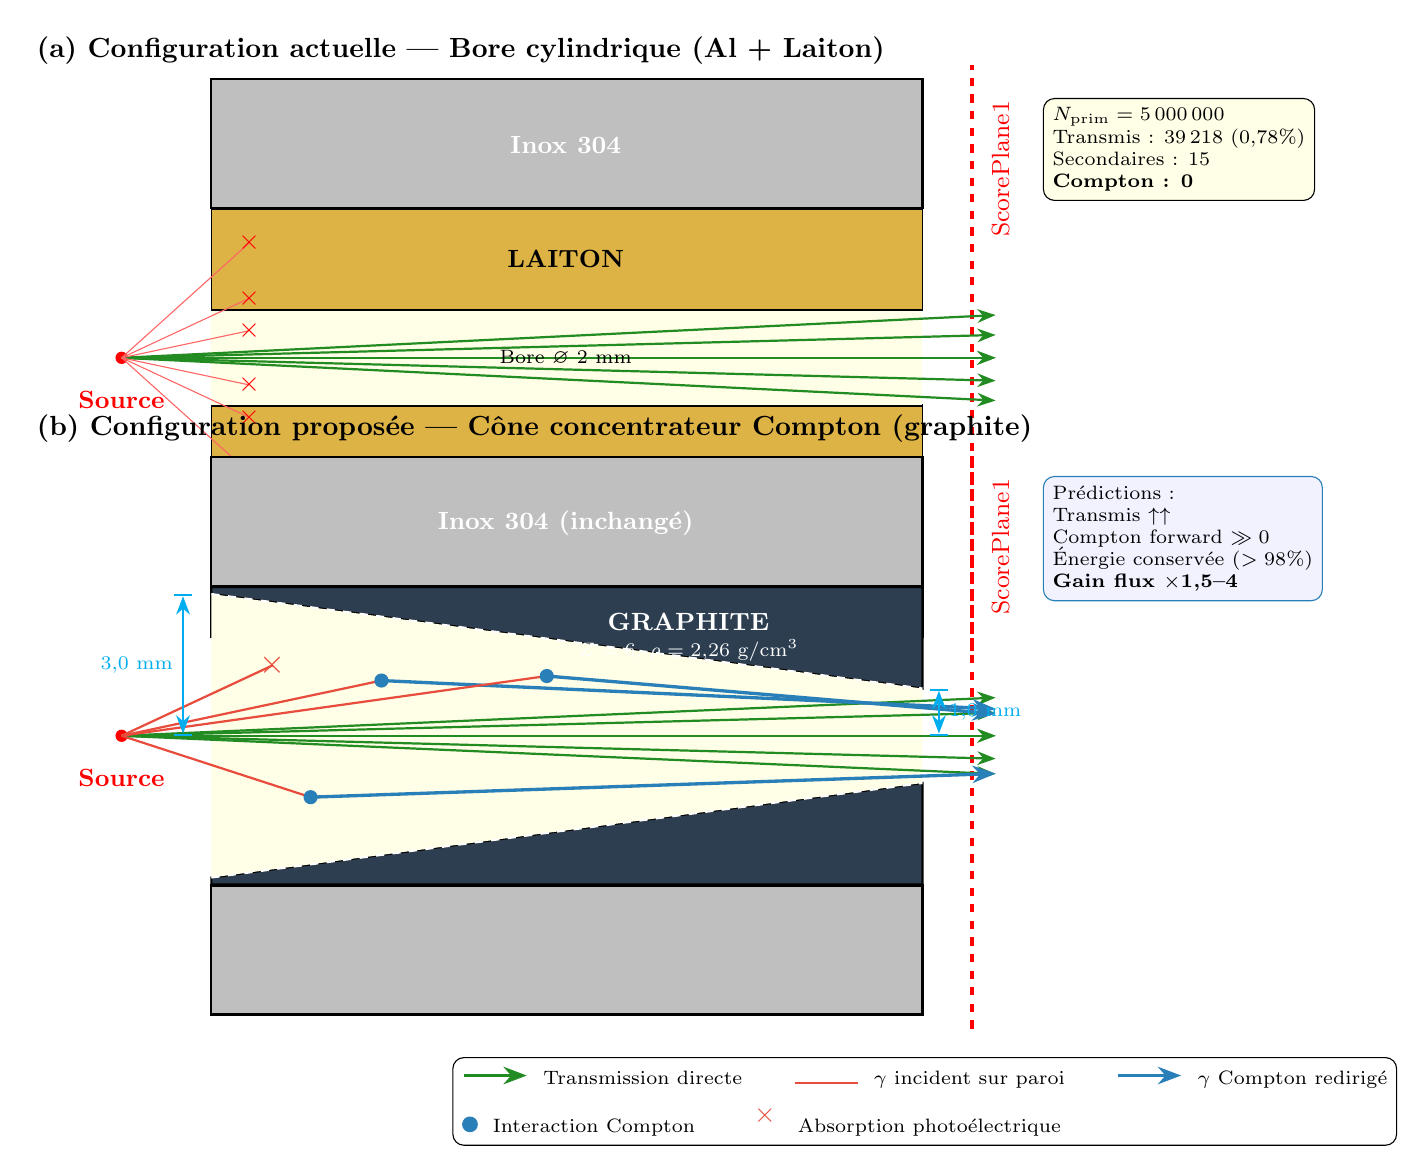
\begin{tikzpicture}[scale=0.60, >=Stealth, every node/.style={font=\footnotesize}]

  % ========== PANEL (a) : CURRENT GEOMETRY ==========
  \begin{scope}[yshift=8cm]
  \node[font=\normalsize\bfseries, anchor=west] at (-2,6.5)
    {(a) Configuration actuelle --- Bore cylindrique (Al + Laiton)};

  % Holder (Inox)
  \foreach \s in {1,-1}{
    \fill[gray!50, draw=black, thick]
      (1.9,\s*3.17) rectangle (16.95,\s*5.9);
    % Brass
    \fill[brass!80, draw=black]
      (1.9,\s*1.024) rectangle (16.95,\s*3.15);
    % Al
    \fill[gray!30, draw=black, thin]
      (1.9,\s*0.999) rectangle (16.95,\s*1.024);
  }
  % Bore
  \fill[yellow!10] (1.9,-0.999) rectangle (16.95,0.999);

  % Source
  \fill[red] (0,0) circle (0.13);
  \node[below, red, font=\small\bfseries] at (0,-0.5) {Source};

  % Scoring plane
  \draw[red, dashed, very thick] (18,-6.2) -- (18,6.2);
  \node[red, rotate=90, font=\small] at (18.6,4) {ScorePlane1};

  % Transmitted rays
  \foreach \a in {0, 1.5, 2.8}{
    \draw[ForestGreen, thick, ->] (0,0) -- ({18.5},{18.5*tan(\a)});
    \draw[ForestGreen, thick, ->] (0,0) -- ({18.5},{-18.5*tan(\a)});
  }
  % Absorbed rays
  \foreach \a in {12, 25, 42}{
    \pgfmathsetmacro{\zhit}{1.9 + 0.8}
    \pgfmathsetmacro{\rhit}{min(\zhit*tan(\a), 3.15)}
    \draw[red!60, thin] (0,0) -- (\zhit,\rhit);
    \node[red, font=\normalsize] at (\zhit,\rhit) {$\times$};
    \draw[red!60, thin] (0,0) -- (\zhit,-\rhit);
    \node[red, font=\normalsize] at (\zhit,-\rhit) {$\times$};
  }

  % Labels
  \node[white, font=\small\bfseries] at (9.4,4.5) {Inox 304};
  \node[font=\small\bfseries] at (9.4,2.1) {LAITON};
  \node[font=\scriptsize] at (9.4,0) {Bore $\varnothing$ 2 mm};

  % Stats box
  \node[draw, fill=yellow!10, rounded corners, align=left, font=\scriptsize,
        anchor=north west] at (19.5,5.5) {%
    $N_{\text{prim}} = 5\,000\,000$ \\
    Transmis : $39\,218$ (0,78\%) \\
    Secondaires : 15 \\
    \textbf{Compton : 0}
  };
  \end{scope}

  % ========== PANEL (b) : PROPOSED GEOMETRY ==========
  \begin{scope}[yshift=0cm]
  \node[font=\normalsize\bfseries, anchor=west] at (-2,6.5)
    {(b) Configuration propos\'ee --- C\^one concentrateur Compton (graphite)};

  % Holder (Inox)
  \foreach \s in {1,-1}{
    \fill[gray!50, draw=black, thick]
      (1.9,\s*3.17) rectangle (16.95,\s*5.9);
  }
  % Graphite cone
  \foreach \s in {1,-1}{
    \fill[graphite, draw=black, thick]
      (1.9,\s*3.0) -- (16.95,\s*1.0) -- (16.95,\s*3.15) -- (1.9,\s*3.15) -- cycle;
  }
  % Conical bore (air)
  \fill[yellow!10]
    (1.9,3.0) -- (16.95,1.0) -- (16.95,-1.0) -- (1.9,-3.0) -- cycle;

  % Inner cone surface (dashed white)
  \draw[white, thick, dashed] (1.9,3.0) -- (16.95,1.0);
  \draw[white, thick, dashed] (1.9,-3.0) -- (16.95,-1.0);

  % Source
  \fill[red] (0,0) circle (0.13);
  \node[below, red, font=\small\bfseries] at (0,-0.5) {Source};

  % Scoring plane
  \draw[red, dashed, very thick] (18,-6.2) -- (18,6.2);
  \node[red, rotate=90, font=\small] at (18.6,4) {ScorePlane1};

  % Direct transmitted rays (green)
  \foreach \a in {0, 1.5, 2.5}{
    \draw[ForestGreen, thick, ->] (0,0) -- ({18.5},{18.5*tan(\a)});
    \draw[ForestGreen, thick, ->] (0,0) -- ({18.5},{-18.5*tan(\a)});
  }

  % Compton ray 1 (upper wall, steep)
  \draw[photored, thick] (0,0) -- (5.5, {5.5*tan(12)});
  \fill[comptonblue] (5.5, {5.5*tan(12)}) circle (0.15);
  \draw[comptonblue, very thick, ->] (5.5, {5.5*tan(12)}) -- (18.5, {5.5*tan(12) - 0.6});

  % Compton ray 2 (upper wall, shallow)
  \draw[photored, thick] (0,0) -- (9, {9*tan(8)});
  \fill[comptonblue] (9, {9*tan(8)}) circle (0.15);
  \draw[comptonblue, very thick, ->] (9, {9*tan(8)}) -- (18.5, {9*tan(8) - 0.8});

  % Compton ray 3 (lower wall)
  \draw[photored, thick] (0,0) -- (4, {-4*tan(18)});
  \fill[comptonblue] (4, {-4*tan(18)}) circle (0.15);
  \draw[comptonblue, very thick, ->] (4, {-4*tan(18)}) -- (18.5, {-4*tan(18) + 0.5});

  % Photo-absorbed ray (upper)
  \draw[photored, thick] (0,0) -- (3.2, {3.2*tan(25)});
  \node[photored, font=\large] at (3.2, {3.2*tan(25)}) {$\times$};

  % Labels
  \node[white, font=\small\bfseries] at (9.4,4.5) {Inox 304 (inchang\'e)};
  \node[white, font=\small\bfseries] at (12,2.4) {GRAPHITE};
  \node[white, font=\scriptsize] at (12,1.8) {$Z = 6$, $\rho = 2{,}26$ g/cm$^3$};

  % Dimensions
  \draw[|<->|, cyan, thick] (1.3,3.0) -- node[left, font=\scriptsize, cyan] {3,0 mm} (1.3,0);
  \draw[|<->|, cyan, thick] (17.3,1.0) -- node[right, font=\scriptsize, cyan] {1,0 mm} (17.3,0);

  % Prediction box
  \node[draw=comptonblue, fill=blue!5, rounded corners, align=left, font=\scriptsize,
        anchor=north west] at (19.5,5.5) {%
    Pr\'edictions : \\
    Transmis $\uparrow\uparrow$ \\
    Compton forward $\gg 0$ \\
    \'Energie conserv\'ee ($>98$\%) \\
    \textbf{Gain flux $\times$1,5--4}
  };

  \end{scope}

  % ========== LEGEND ==========
  \node[draw, fill=white, rounded corners, align=left, font=\scriptsize,
        anchor=north west] at (7,-6.8) {%
    \tikz\draw[ForestGreen, very thick, ->] (0,0) -- (0.8,0);
      ~Transmission directe \qquad
    \tikz\draw[photored, thick] (0,0) -- (0.8,0);
      ~$\gamma$ incident sur paroi \qquad
    \tikz\draw[comptonblue, very thick, ->] (0,0) -- (0.8,0);
      ~$\gamma$ Compton redirig\'e \\[3pt]
    \tikz\fill[comptonblue] (0.1,0.1) circle (0.1);
      ~Interaction Compton \qquad
    \tikz\node[photored, font=\normalsize] {$\times$};
      ~Absorption photo\'electrique
  };

\end{tikzpicture}%
}% end resizebox
\caption{Coupe longitudinale $(r, z)$ des deux configurations.
  \textbf{(a)}~Syst\`eme actuel~: tous les photons hors du c\^one g\'eom\'etrique
  \'etroit sont absorb\'es dans le laiton.
  \textbf{(b)}~C\^one graphite~: le bore conique intercepte les photons \`a angle
  interm\'ediaire, les diffuse par Compton et les redirige vers le plan de scoring.}
\label{fig:schema}
\end{figure}

\subsection{Param\`etres g\'eom\'etriques}

Le c\^one s'inscrit dans le volume libre \`a l'int\'erieur du porte-collimateur
($R_{\text{int}} = \SI{3,17}{\milli\metre}$). Le tableau~\ref{tab:cone_params} donne les
dimensions.

\begin{table}[H]
\centering
\caption{Param\`etres g\'eom\'etriques du c\^one concentrateur.}
\label{tab:cone_params}
\renewcommand{\arraystretch}{1.15}
\begin{tabular}{@{}l c l@{}}
\toprule
\textbf{Param\`etre} & \textbf{Valeur} & \textbf{Description} \\
\midrule
\multicolumn{3}{@{}l}{\textit{Bore conique (surface interne)}} \\
$R_{\text{in,entr\'ee}}$ & \SI{3,0}{\milli\metre} & Rayon c\^ot\'e source (large) \\
$R_{\text{in,sortie}}$   & \SI{1,0}{\milli\metre} & Rayon c\^ot\'e d\'etecteur (\'etroit) \\
Demi-angle du c\^one     & 7,6$^\circ$ &
  $\alpha = \arctan\!\dfrac{R_{\text{in,e}} - R_{\text{in,s}}}{L}$ \\[6pt]
\midrule
\multicolumn{3}{@{}l}{\textit{Enveloppe ext\'erieure}} \\
$R_{\text{ext}}$ & \SI{3,15}{\milli\metre} &
  $= R_{\text{int,inox}} - \SI{0,02}{\milli\metre}$ (jeu) \\
\midrule
\multicolumn{3}{@{}l}{\textit{Dimensions axiales}} \\
$z_{\text{d\'ebut}}$   & \SI{1,90}{\milli\metre} & Face c\^ot\'e source \\
$z_{\text{fin}}$       & \SI{16,95}{\milli\metre} & Face c\^ot\'e d\'etecteur \\
Longueur               & \SI{15,05}{\milli\metre} & \\
\midrule
\multicolumn{3}{@{}l}{\textit{\'Epaisseur de paroi}} \\
C\^ot\'e entr\'ee      & \SI{0,15}{\milli\metre} & Mince --- photons \`a grand angle traversent \\
C\^ot\'e sortie        & \SI{2,15}{\milli\metre} & \'Epaisse --- bonne probabilit\'e d'interaction \\
\midrule
Mat\'eriau Geant4      & \texttt{G4\_GRAPHITE} & Carbone, $\rho = \SI{2,26}{\gram\per\centi\metre\cubed}$ \\
\bottomrule
\end{tabular}
\end{table}

\subsection{Incidence rasante et chemin optique effectif}

Un aspect essentiel de la g\'eom\'etrie conique est l'\textbf{effet d'incidence rasante}~:
les photons \`a angle interm\'ediaire frappent la surface interne du c\^one sous un angle
tr\`es faible par rapport \`a la surface, ce qui augmente consid\'erablement le chemin
optique dans le graphite. Sch\'ematiquement~:

\begin{center}
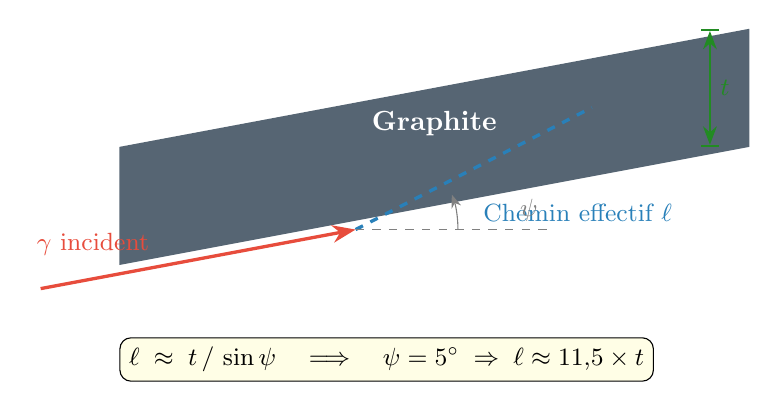
\begin{tikzpicture}[scale=1.0, >=Stealth]
  % Graphite wall (thick slab, tilted)
  \fill[graphite!80] (0,0) -- (8,1.5) -- (8,3.0) -- (0,1.5) -- cycle;
  \node[white, font=\bfseries] at (4,1.8) {Graphite};

  % Incoming ray (grazing)
  \draw[photored, very thick, ->] (-1,-0.3) -- (3,0.45);
  \node[photored, font=\small, above left] at (0.5,0) {$\gamma$ incident};

  % Path through wall
  \draw[comptonblue, very thick, dashed] (3,0.45) -- (6,2.0);
  \node[comptonblue, font=\small, below right] at (4.5,0.9)
    {Chemin effectif $\ell$};

  % Radial thickness
  \draw[|<->|, ForestGreen, thick] (7.5,1.5) -- node[right, font=\small] {$t$} (7.5,3.0);

  % Angles
  \draw[gray, thin, dashed] (3,0.45) -- (5.5,0.45);
  \draw[gray, ->] (4.3,0.45) arc[start angle=0, end angle=20, radius=1.3];
  \node[gray, font=\small] at (5.2,0.7) {$\psi$};

  % Formula
  \node[draw, fill=yellow!10, rounded corners, font=\small, anchor=west] at (0,-1.2)
    {$\ell \;\approx\; t \,/\, \sin\psi \quad\Longrightarrow\quad
      \psi = 5^\circ \;\Rightarrow\; \ell \approx 11{,}5 \times t$};
\end{tikzpicture}
\end{center}

\noindent Pour un photon \'emis \`a $\theta \approx 8^\circ$ (proche du demi-angle du c\^one
$\alpha = 7{,}6^\circ$), l'angle d'incidence sur la paroi est
$\psi = \theta - \alpha \approx 0{,}4^\circ$, donnant un chemin de plusieurs centim\`etres
dans le graphite~! Cela augmente dramatiquement la probabilit\'e d'interaction Compton.

% ======================================================================
\section{Estimation quantitative du gain}
\label{sec:estimate}
% ======================================================================

\subsection{Bilan des photons}

Pour \num{5000000} photons primaires~:

\begin{table}[H]
\centering
\caption{Budget de photons estim\'e pour le c\^one graphite.}
\label{tab:budget}
\begin{tabular}{@{}l r l@{}}
\toprule
\textbf{Cat\'egorie} & \textbf{Estimation} & \textbf{Note} \\
\midrule
Transmis direct ($\theta < 3{,}2^\circ$)
  & $\sim$\num{39000} & Identique \`a la r\'ef\'erence \\[4pt]
Interceptent le c\^one ($3{,}2^\circ < \theta < 30^\circ$)
  & $\sim$\num{130000} & Grande acceptance angulaire \\
\quad$\to$ Compton forward & $\sim$\numrange{2500}{15000} & Redirig\'es vers le plan \\
\quad$\to$ Photo-absorb\'es & $\sim$\numrange{25000}{75000} & Perdus dans le graphite \\
\quad$\to$ Traversent la paroi & $\sim$\numrange{50000}{100000} & Absorb\'es par l'inox \\[4pt]
Grand angle ($\theta > 30^\circ$)
  & $\sim$\num{4830000} & Absorb\'es (inox + graphite) \\
\midrule
\textbf{Total sur ScorePlane1}
  & $\sim$\numrange{42000}{54000} & \textbf{Gain $\times 1{,}1$ \`a $\times 1{,}4$} \\
\bottomrule
\end{tabular}
\\[6pt]
\footnotesize\textit{Note~: ces estimations sont analytiques et approximatives.
Seule la simulation Monte Carlo donnera la r\'eponse d\'efinitive.}
\end{table}

\begin{figure}[H]
\centering
\includegraphics[width=\textwidth]{fig_gain_estimation.pdf}
\caption{\textbf{(a)}~Acceptance angulaire~: le c\^one graphite capture les photons
  jusqu'\`a $\sim$58$^\circ$ (quasi-totalit\'e du c\^one d'\'emission), alors que le bore
  actuel ne laisse passer que $\theta < 4{,}9^\circ$.
  \textbf{(b)}~Budget de flux estim\'e pour 5M primaires. Le gain principal vient des
  photons Compton forward et de la fuite \`a travers la paroi mince.}
\label{fig:gain}
\end{figure}

\subsection{Comparaison synth\'etique}

\begin{table}[H]
\centering
\caption{R\'ef\'erence actuelle vs c\^one graphite (pr\'edictions).}
\label{tab:comparison}
\renewcommand{\arraystretch}{1.2}
\begin{tabular}{@{}>{\bfseries}p{4cm} c c@{}}
\toprule
 & \textbf{R\'ef\'erence} & \textbf{C\^one graphite} \\
 & (Al + Laiton) & (pr\'edit) \\
\midrule
Collimateur   & Cylindre $\varnothing$ 3\,mm & C\^one 6$\to$2\,mm \\
Mat\'eriau    & Al ($Z{=}13$) + Laiton ($Z{\approx}29$) & Graphite ($Z{=}6$) \\
Transmis/5M   & \num{39218} & $\sim$\numrange{42000}{54000} \\
Taux transm.  & 0,78\% & $\sim$0,8--1,1\% \\
Compton       & \textbf{0} & $\gg 0$ \\
$\Delta E$ Compton & --- & $< 2$\% \`a 10\,keV \\
Dose eau      & 31,4 nGy & $\uparrow$ attendu \\
\bottomrule
\end{tabular}
\end{table}

% ======================================================================
\section{Impl\'ementation Geant4}
\label{sec:implementation}
% ======================================================================

L'impl\'ementation n\'ecessite trois modifications minimales dans le code existant~:

\begin{table}[H]
\centering
\caption{Modifications apport\'ees au code source Geant4.}
\label{tab:code}
\small
\begin{tabular}{@{}c l p{7.5cm}@{}}
\toprule
\textbf{\#} & \textbf{Fichier} & \textbf{Modification} \\
\midrule
1 & \texttt{.hh} & Ajout du membre \texttt{G4Material* MyGraphite} \\
2 & \texttt{.cc}, \texttt{DefineMaterial()} & Chargement de
    \texttt{"G4\_GRAPHITE"} via le NIST Manager \\
3 & \texttt{.cc}, \texttt{ConstructGDML()} & Remplacement des sections
    Al\,3\,mm et Laiton\,3\,mm par un \texttt{G4Cons} param\'etrique \\
\bottomrule
\end{tabular}
\end{table}

Le solide \texttt{G4Cons} (c\^one tronqu\'e creux) est d\'efini par~:
\begin{verbatim}
  new G4Cons("solidConeCompton",
    coneRinEntry,  coneRout,    // Rmin1, Rmax1 (source)
    coneRinExit,   coneRout,    // Rmin2, Rmax2 (détecteur)
    coneHalfLen, 0.*deg, 360.*deg);
\end{verbatim}

\noindent Pour tester un autre mat\'eriau, il suffit de modifier une seule ligne~:
\begin{verbatim}
  G4Material* coneMaterial = MyGraphite;
  // Alternatives :
  // -> nist->FindOrBuildMaterial("G4_PLEXIGLASS");
  // -> nist->FindOrBuildMaterial("G4_POLYETHYLENE");
  // -> nist->FindOrBuildMaterial("G4_BORON_CARBIDE");
\end{verbatim}

% ======================================================================
\section{Indicateurs de succ\`es pour le run Geant4}
\label{sec:indicators}
% ======================================================================

\noindent\fbox{\parbox{0.97\linewidth}{
\textbf{Check-list d'analyse apr\`es le run avec c\^one graphite~:}
\begin{enumerate}[nosep,leftmargin=2em]
  \item \textbf{Flux total sur ScorePlane1} --- comparer \`a la r\'ef\'erence (\num{39218}/5M).
  \item \textbf{Lignes \texttt{[SECONDARY\_ORIGIN]}} --- rechercher
    \texttt{creator\_process: compt} avec
    \texttt{vertex\_volume: logicConeCompton}.
    Leur nombre doit \^etre $\gg 15$.
  \item \textbf{Budget \texttt{[LOSS][BY-MAT]}} --- le laiton et l'aluminium doivent
    dispara\^itre, remplac\'es par \texttt{G4\_GRAPHITE} et
    \texttt{StainlessSteel304}.
  \item \textbf{Spectre en \'energie} --- les Compton forward doivent appara\^itre \`a
    $E \gtrsim 0{,}98 \times E_{\text{incident}}$, l\'eg\`erement d\'ecal\'es.
  \item \textbf{Distribution radiale} --- les Compton redirig\'es cr\'eeront un
    \textbf{halo} autour du faisceau direct.
  \item \textbf{Dose dans l'eau} --- gain attendu dans les anneaux centraux.
\end{enumerate}
}}

\end{document}
